\chapter{Desarrollo}\label{chapter:desarrollo}

En este capítulo se dan detalles sobre el proceso de desarrollo del proyecto, el cual se ha dividido en dos fases. La primera fase ha consistido en hacer un experimento piloto, en el que se ha puesto a prueba una propuesta inicial del entorno de pádel para estudiar su viabilidad. En la segunda fase se ha implementado la versión definitiva de este entorno, la cual ha derivado de la resolución de los problemas surgidos durante la primera fase.

\section{Experimento piloto}

\subsection{Reglamento del entorno virtual}

Para diseñar el entorno virtual de pádel, el primer paso fue definir una normativa lo más parecida posible al entorno real:
\begin{enumerate}
    \item[-] Un partido de pádel se divide normalmente en tres sets. En el entorno virtual, al tratarse de una simulación, consiste en un único set que se juega indefinidamente, es decir, se ignora la puntuación de juegos.
    \item[-] A diferencia de un partido real, en el entorno virtual no se permite jugar fuera de la pista, por lo que si la pelota se sale fuera se considera falta.
    \item[-] Cada juego se forma con puntos: el primer punto que gana una pareja suma 15 puntos, el segundo 30, el tercero 40 y con el cuarto se gana un juego. Cuando se produce un empate a 40 puntos, gana el juego la pareja que sume dos puntos de ventaja.
    \item[-] Durante un juego el servicio lo realiza siempre el mismo jugador. El servicio empieza en el lateral derecho de la pista, y se va alternando de lado tras cada punto.
    \item[-] Tras un juego se produce una rotación en el servicio. Dado los jugadores A, B, C y D, formando las parejas AB y CD, el orden de saque sería A $\rightarrow$ C $\rightarrow$ B $\rightarrow$ D $\rightarrow$ A.
    \item[-] En el servicio, el jugador debe botar la pelota detrás de la línea de saque y enviar la pelota de manera que el primer rebote sea en el lado contrario del campo rival, sin sobrepasar la línea de saque del rival. Tras el primer rebote en el suelo, la pelota no puede tocar la malla. No cumplir estas condiciones se considera falta.
    \item[-] A la hora de devolver la pelota, se permite golpear la pelota contra la pared del propio campo. Tras un golpeo contra la pared o un golpeo directo, si la pelota rebota por primera vez en el propio campo o en la pared se considera falta.
    \item[-] Tras devolver la pelota, esta puede rebotar como máximo una vez en el suelo. El número de rebotes en la pared es indiferente. Si una pelota rebota dos veces en el suelo, el equipo que haya enviado esa pelota gana un punto.
    \item[-] Tras devolver la pelota, si la pelota impacta en el compañero o la red es punto para el rival. Si la pelota impacta en alguno de los dos oponentes, es punto para el propio equipo.
\end{enumerate}

\subsection{Diseño inicial}
Una vez establecidas las reglas, lo siguiente fue diseñar la pista de pádel en Unity, partiendo del diseño de una pista oficial de World Padel Tour. Al no tratarse de un TFG enfocado en gráficos, bastaba con un diseño simple pero funcional. En la Figura~\ref{fig:pista-padel} se muestra la pista de pádel del entorno virtual, la cual sigue las medidas oficiales de una pista de pádel, y tiene paredes compuestas por materiales que representan vidrio templado (en blanco transparente) y mallas metálicas (en negro transparente), además de una red en el centro. Las paredes tienen un \emph{Physic Material} con la propiedad $\emph{Dynamic Friction}=$ 0.5, para que la pelota pierda velocidad con cada rebote.

El origen de coordenadas local $(0,0)$ para un entorno se sitúa en el centro de la pista, de manera que el rango de la pista es $x \in [-5, 5]$ en el eje $X$, y $z \in [-10, 10]$ en el eje $Z$.

En cuanto a pelota, la idea original era utilizar medidas reales, pero finalmente se optó por utilizar medidas más grandes por cuestiones de visibilidad. La pelota tiene un \emph{Physic Material} con $\emph{Bounciness}=$ 0.77, de manera que tras caer desde una altura de 2.5 metros, la pelota rebota y alcanza una altura de 1.5 metros. También se le ha atribuido un \emph{Trail Renderer} utilizado para visualizar su trayectoria y saber qué equipo ha sido el último en golpearla.

Los jugadores, sobre los cuales se implementan los agentes, tienen forma de cápsula y tienen el color correspondiente a su equipo: naranja para el equipo denominado T1, y morado para el equipo denominado T2. Para poder diferenciar entre los compañeros del mismo equipo, se les ha añadido una cinta blanca para el Jugador 1 y una cinta negra para el Jugador 2. Los agentes tienen un alcance de 2 metros de radio para golpear la pelota.

Además, a cada \emph{Game Object} se le han añadido los componentes necesarios para simular las físicas mediante el motor de físicas de Unity (\emph{Colliders} y \emph{Rigid Bodies}).

\begin{figure}[H]
    \centering
    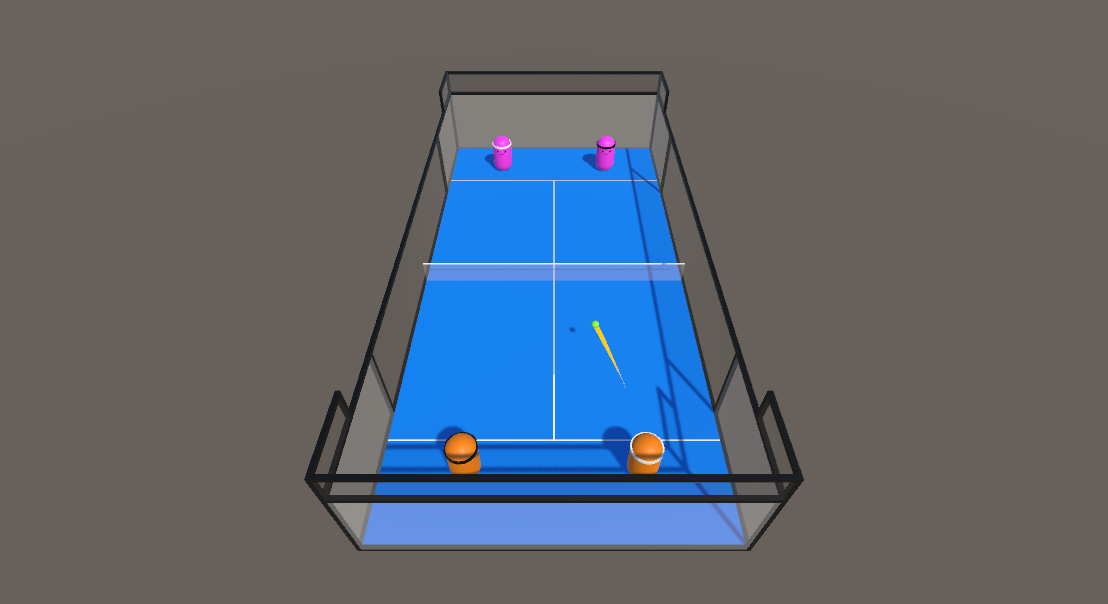
\includegraphics[width=\textwidth]{figures/pista-padel.png}
    \caption[Entorno virtual de pádel en Unity]{Entorno virtual de pádel en Unity. (Elaboración propia)}
    \label{fig:pista-padel}
\end{figure}

\subsection{Implementación inicial}

La implementación de la lógica detrás de los elementos definidos consiste principalmente en tres \emph{Scripts}, uno para controlar el entorno, otro para la pelota y otro para definir el agente vinculado a cada jugador. En esta sección se da una idea general sobre cómo funcionan estos componentes, ya que se trata de una implementación inicial que acabó pasando por muchos cambios.

\subsubsection{Controlador del entorno}

El controlador del entorno se encarga de la lógica detrás del flujo de un partido de pádel: puntuaciones, servicio y rotaciones de los jugadores, cumpliendo con las reglas establecidas anteriormente. En la Figura \ref{fig:padel-flow-chart} se muestra un diagrama de flujo simplificado del trascurso de un partido de pádel en el entorno virtual.

Se optó por implementar el servicio a mano, utilizando valores fijos para la posición y la fuerza de golpeo, ya que aprender estrategias para el saque no es muy relevante para este proyecto.

\subsubsection{Controlador de la pelota}

El controlador de la pelota gestiona el estado de la pelota: qué equipo ha golpeado, cuántas veces ha rebotado, dónde ha rebotado, además de definir métodos para golpear la pelota. Este controlador se comunica con el controlador del entorno para incrementar la puntuación de un equipo, ya sea debido a una falta o el doble rebote en el suelo de la pelota.

\subsubsection{Agente de pádel}

El agente, el cual controla el jugador con el que está vinculado, tiene definidos los elementos que requiere ML-Agents para utilizar algoritmos de aprendizaje por refuerzo. Estos elementos son el espacio de observaciones, el espacio de acciones, las recompensas y el principio y fin de un episodio.

El espacio de observaciones de un agente consiste en un total de 14 parámetros:
\begin{enumerate}
    \item[-] Posición local 2D del propio agente, su compañero y los dos oponentes.
    \item[-] Posición local y velocidad 3D de la pelota.
\end{enumerate}

El espacio de acciones está formado por:
\begin{enumerate}
    \item[-] 3 acciones continuas, utilizadas para controlar la fuerza de golpeo.
    \item[-] 4 acciones discretas, utilizadas para el tipo de golpeo, el movimiento lateral, el movimiento frontal y el giro. En ML-Agents, una rama consiste.
\end{enumerate}

Las recompensas definidas son +1 por cada pelota devuelta y -1 por cada punto que se pierde. El comportamiento que se quería buscar con esta configuración era que los agentes pudieran mantener la pelota en juego.

En el entorno virtual, un episodio consiste en un punto de un juego: empieza con el servicio y termina con la obtención de un punto para cualquier equipo.

\begin{figure}[H]
    \centering
    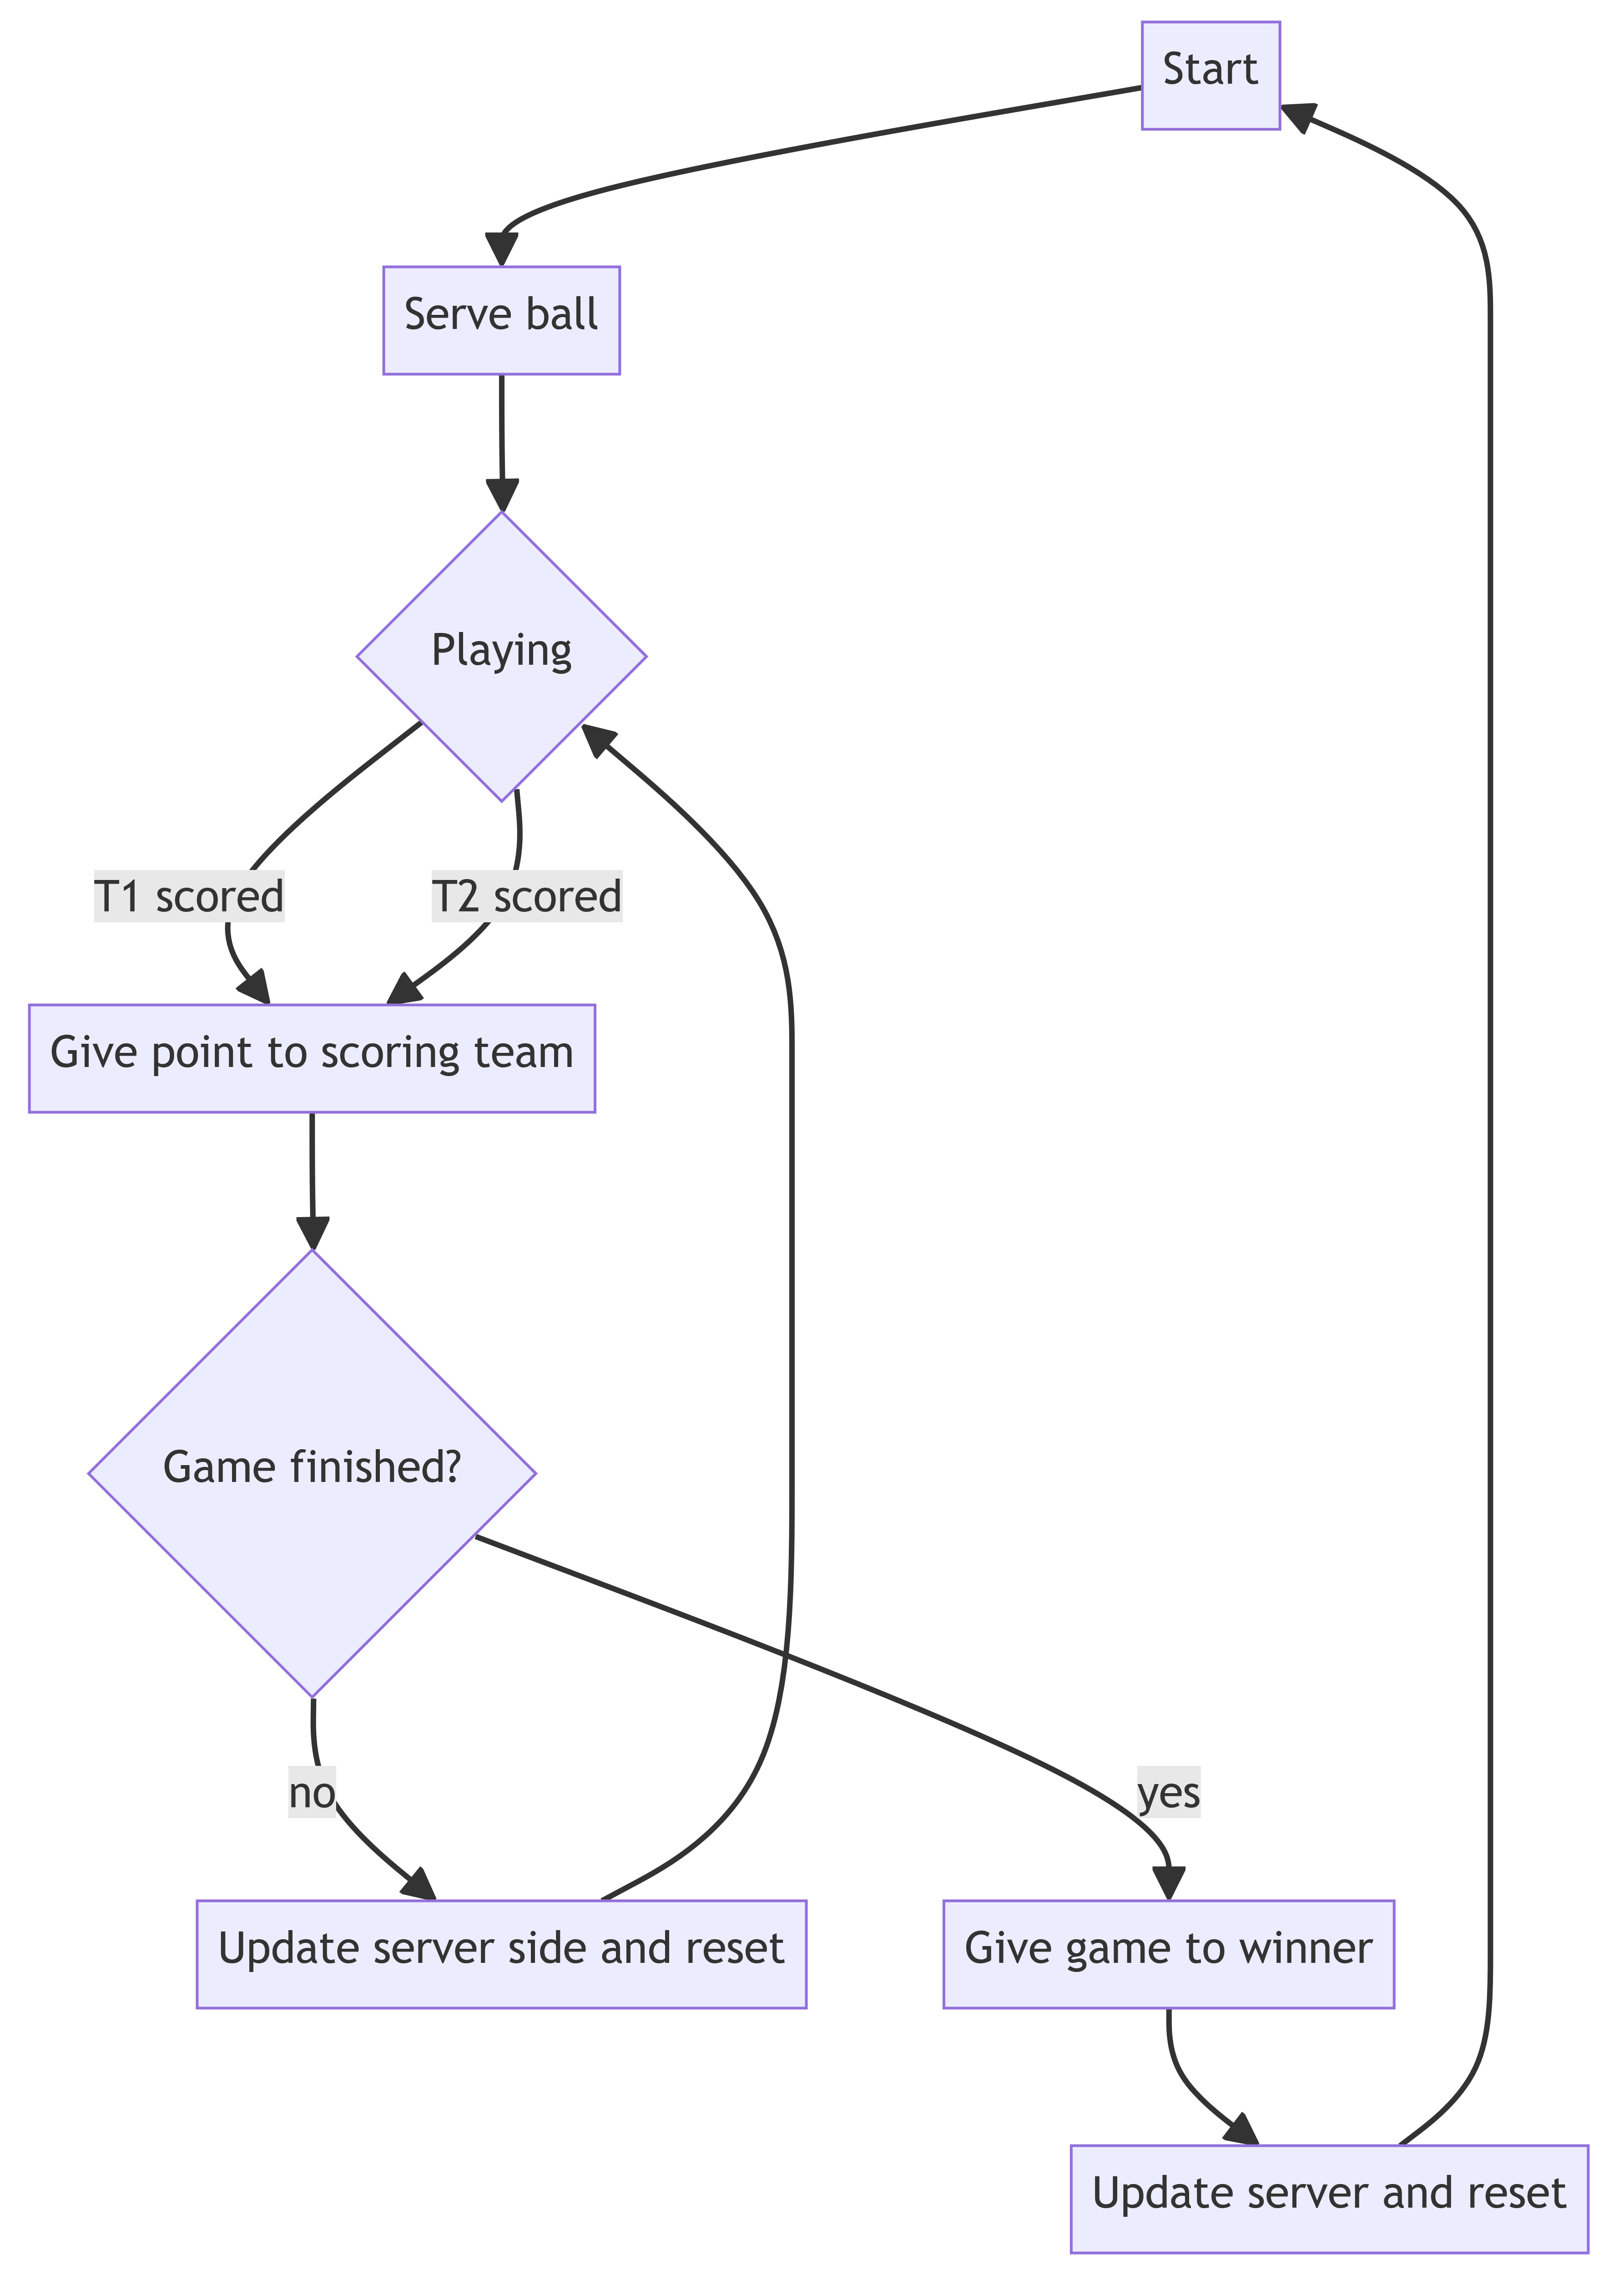
\includegraphics[width=10cm]{figures/flow-chart.png}
    \caption[Diagrama de flujo simplificado del entorno virtual de pádel]{Diagrama de flujo simplificado del entorno virtual de pádel. (Elaboración propia)}
    \label{fig:padel-flow-chart}
\end{figure}

\subsection{Problemas de la versión inicial}

Al principio de esta memoria, uno de los objetivos principales que se definió para este proyecto era la simplicidad en la implementación de la lógica detrás de un partido de pádel. Por lo tanto, la filosofía que se siguió durante los primeros experimentos fue ``cuanto más simple, mejor''.

En un modelo ideal, los agentes deberían ser capaces de aprender a golpear la pelota con la fuerza necesaria para enviarla a la posición que maximice la probabilidad de ganar un punto. En una primera prueba, en la cual los agentes eran libres de emplear una fuerza cualquiera, siempre y cuando estuviera dentro de un rango válido, por muchas horas de entrenamiento que se hacían, los agentes no eran siquiera capaces de enviar la pelota al campo rival.

\newpage

Tras esta primera prueba, se hizo evidente que era necesario hacer cambios en el comportamiento del agente, simplificando el espacio de acciones. Esta vez, la idea era hacer que el agente aprendiera a modificar fuerzas de golpeo predefinidas, según el tipo de golpeo (globo, derecha, remate...), mediante acciones continuas, como si añadieran un cierto margen de error en la fuerza. Aunque los resultados fueron positivos, el comportamiento de los agentes no era el deseado, ya que en realidad los agentes no podían elegir voluntariamente hacia dónde enviar la pelota, sino que debían partir siempre de una fuerza fija, resultando en un entorno muy poco realista.

Llegados hasta ese punto, la propuesta final fue deshacerse de las acciones continuas, ya que estaba claro que era más sencillo elegir sobre un rango discreto que no sobre uno continuo, por lo que este cambio facilitaría bastante el aprendizaje. Pero, ¿cómo se debería modelar el espacio de acciones, limitándose a acciones discretas, para conseguir un comportamiento realista? La solución más directa fue dividir la pista en posiciones equidistantes, de manera que el agente pudiera elegir hacia qué posición enviar la pelota, y dejar el cálculo de la fuerza al propio entorno. Esto se asemeja al comportamiento de un jugador de pádel: primero decide el tipo de acción a realizar, que incluye tipo de golpe y dirección del mismo (aspectos tácticos), y luego realiza los movimientos necesarios para ejecutar esa decisión (aspectos técnicos).

Otra cuestión importante a resolver era el posicionamiento de los agentes. En la primera versión del entorno, las recompensas definidas eran demasiado escasas. Esto hacía que los agentes, al no recibir ninguna retroalimentación entre devoluciones de la pelota, se movieran hacia la pelota aunque el compañero ya se encontrara cerca, y mantenían muy poca distancia entre sí, dejando demasiados espacios libres en la pista. El comportamiento ideal hubiera sido que los jugadores cubrieran posiciones óptimas dada cada situación de un partido de pádel. Por este motivo, de cara a la versión definitiva, era necesario cambiar la función de recompensas para poder guiar a los agentes durante los momentos en los que no disponen de una valoración de cómo están actuando.

Al requerir más funcionalidades, era inviable mantener toda la lógica necesaria en los tres \emph{scripts} definidos. Debido a esto, de cara a la versión definitiva, otro objetivo que se planteó fue repartir cada funcionalidad en un \texttt{Script} específico. Por ejemplo, el control de la puntuación, el servicio y la rotación de los jugadores recaía únicamente en el controlador del entorno. Tras el rediseño, tendría que haber un \texttt{Script} para cada funcionalidad, y se utilizaría el controlador del entorno como intermediario entre estos componentes.

\section{Versión final del entorno virtual}

\subsection{Diseño final}

Tras los problemas de la versión inicial, los cambios que se hicieron fueron los siguientes:

\begin{enumerate}
    \item[-] El primer cambio consistió en reestructurar la implementación de los controladores ya existentes. El controlador del entorno debía servir como mediador entre el resto de controladores. A partir de ahí, cada funcionalidad debía tener su propio controlador: control de la pelota, el servicio y la puntuación.
    \item[-] La funcionalidad principal que se añadió fue el cálculo de fuerzas para enviar la pelota hacia una posición en concreto. Para discretizar estas posiciones, se optó por dividir el campo de cada equipo en una cuadrícula de tamaño $5 \times 5$.
    \item[-] Recordando que el origen de coordenadas local $(0,0)$ de una pista se sitúa en el centro de la pista, y al ser el pádel un juego simétrico, es posible simplificar el espacio de observaciones invirtiendo los ejes X y Z de los agentes de uno de los dos equipos. De esta manera, la política tendría que aprender a jugar únicamente en uno de los dos campos. Esto es válido ya que la decisión óptima en un campo debería ser la misma en el otro, cuando el estado es equivalente. Por ello, el espacio de observaciones se modificó de manera que los agentes del equipo T2 perciben ahora las posiciones con los ejes invertidos.
    \item[-] En cuanto al espacio de acciones de los agentes, en la primera versión se utilizaba un \texttt{Rigidbody} y el movimiento se basaba en aplicarle fuerzas y rotaciones. Esto no parecía funcionar muy bien, por lo que el \texttt{Rigid Body} se sustituyó por un \texttt{Character Controller}, y las acciones consisten ahora en moverse hacia delante, detrás, izquierda o derecha.
    \item[-] Para evitar la escasez de recompensas, se han añadido unas guías denominadas ``posiciones clave''. Estas posiciones consisten en posiciones de interés que recompensan a los agentes cuando están cerca o bien se están acercando a la posición en cuestión.
    \item[-] Las posiciones clave introducen la necesidad de asignar roles a cada agente, ya que la función de recompensa cambia según la situación del partido. Por ejemplo, en un mismo campo, las posiciones de interés cambian según si los agentes deben devolver una pelota, o si están esperando a que los oponentes la devuelvan.
    \item[-] Cuantas más funcionalidades tiene una aplicación, más probabilidades hay de que surjan errores durante el desarrollo. Por ello, también se añadieron herramientas para realizar una depuración de una manera cómoda.
\end{enumerate}

El diseño del entorno se mantuvo igual que en la versión inicial, pero se añadieron todos los elementos visuales necesarios para crear un modo de depuración, mostrado en la Figura \ref{fig:pista-padel-debug}.  Esto incluye el uso de textos para mostrar la puntuación y la información de los agentes, los roles y la pelota; \texttt{Prefabs} para materializar los puntos clave; marcas en los jugadores que indican los roles que tienen asignados; y un \texttt{Line Renderer} que permite simular la trayectoria de la pelota.

\begin{figure}[H]
    \centering
    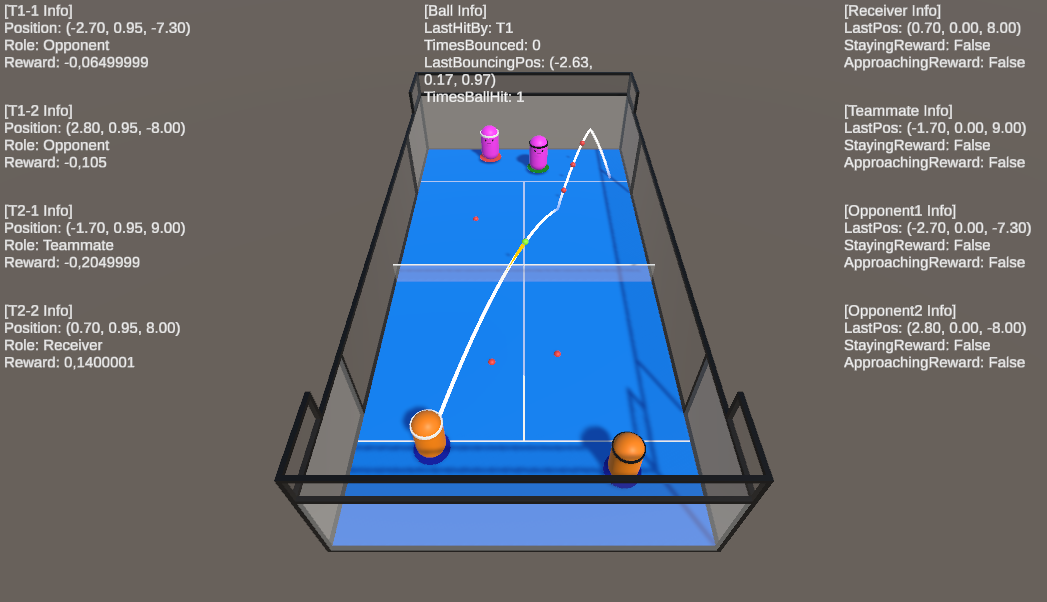
\includegraphics[width=13cm]{figures/pista-padel-debug.png}
    \caption[Entorno virtual de pádel con el modo de depuración activado]{Entorno virtual de pádel con el modo de depuración activado. (Elaboración propia)}
    \label{fig:pista-padel-debug}
\end{figure}

\subsection{Implementación final}\label{section:implementacion-final}

En la implementación final se ven reflejados los cambios mencionados previamente. Además de los controladores ya existentes (del entorno, de la pelota, del servicio y de la puntuación), se han añadido más controladores para la implementación de las nuevas funcionalidades. El código fuente de este proyecto está disponible en Github \cite{padel-project}.

\subsubsection{Controlador del entorno}

Como ya se ha mencionado previamente, el controlador del entorno hace de mediador entre el resto de controladores, de manera que cuando un controlador necesita información de otro controlador, debe enviar una solicitud al controlador del entorno para que se encargue de resolverla. Utilizando este patrón de diseño se eliminan las dependencias entre controladores, haciendo que la funcionalidad de cada controlador esté aislada y el mantenimiento sea más sencillo.

También se definen enumeraciones y variables públicas que comparten varios elementos del entorno. Las enumeraciones definidas son:
\begin{enumerate}
    \item[-] \texttt{PlayerId}, para dar un identificador a cada jugador.
    \item[-] \texttt{Side}, para representar el lado derecho e izquierdo.
    \item[-] \texttt{Team}, para especificar a qué equipo pertenece cada jugador.
    \item[-] \texttt{Role}, para asignar al agente un rol según sea \texttt{Receiver}, \texttt{Teammate} o \texttt{Opponent}.
\end{enumerate}
Las variables por otra parte, se utilizan para definir las recompensas del entorno:
\begin{enumerate}
    \item[-] \texttt{WinningReward} es la recompensa por ganar un punto.
    \item[-] \texttt{LosingReward} es la recompensa por perder un punto.
    \item[-] \texttt{ApproachingKeyPositionReward} es la recompensa por acercarse a una posición de interés.
    \item[-] \texttt{StayingAroundKeyPositionReward} es la recompensa por quedarse cerca de una posición de interés.
    \item[-] \texttt{HittingBallReward} es la recompensa por darle a la pelota.
\end{enumerate}

Otras variables que tienen un uso más específico son \texttt{DebugMode}, utilizado para activar o desactivar el modo depuración mediante la tecla asignada; \texttt{EnvironmentId}, para asignar un identificador al entorno, ya que se utilizan varios a la vez para el entrenamiento; y \texttt{SimulationCompleted}, para saber si la simulación de la trayectoria de la pelota ha finalizado. 

El resto de variables y métodos definidos son aquellos relacionados con los controladores, necesarios para delegar las solicitudes recibidas al controlador correspondiente.

\newpage

\subsubsection{Controlador del servicio}

El controlador del servicio se encarga de mantener un control sobre el estado del servicio en el comienzo de cada punto. Las principal funcionalidad que tiene consiste en hacer botar la pelota y acto seguido realizar el saque.

Durante el servicio, el primer paso es botar la pelota aplicándole una fuerza vertical negativa. Una vez la pelota haya alcanzado una altura superior a 1 metro tras el rebote, el controlador procede a enviar una solicitud al controlador de la pelota para enviar la pelota a una determinada posición de la cuadrícula de la pista, dependiendo de qué equipo realiza el servicio y desde qué lado.

Como en esta versión aprender a realizar el servicio no es parte del objetivo de aprendizaje, se trata de un proceso determinista en el que, al principio de cada punto, todos los agentes se sitúan en las mismas posiciones, sin moverse, y la pelota se coloca dependiendo de desde dónde se hace el servicio, pero siempre se sitúa a la misma distancia del servidor.

Tras haber realizado el saque, los agentes ya pueden moverse libremente y empieza el punto, el cual se controla a través del controlador de la pelota. Cada vez que finaliza un punto, se realiza la rotación del servicio actualizando las variables pertinentes y se repite el proceso.

\subsubsection{Controlador de la puntuación}

El controlador de la puntuación gestiona los puntos conseguidos por los equipos T1 y T2. Cuando un equipo gana un punto, suma los puntos correspondientes según la puntuación actual (siguiendo el orden 0, 15, 30, 40). Cuando un equipo gana un punto teniendo una puntuación de 40, si el equipo rival no ha llegado a 40 puntos, gana el juego. En el caso de que el equipo rival también tenga 40 puntos, si el equipo rival había ganado un punto de ventaja tras los iguales, ambos equipos vuelven a estar iguales. Un equipo gana un punto de ventaja cuando el equipo rival no tiene ninguno, y gana el juego tras dos puntos de ventaja seguidos.

Cuando termina un punto, el controlador de la puntuación envía una solicitud al controlador del entorno para cambiar el lado del servicio (izquierda o derecha del equipo correspondiente), y seguidamente otra solicitud para reiniciar el entorno. Cuando termina un juego, envía una solicitud al controlador del entorno para efectuar la rotación del servicio, el cual empieza desde el lado derecho del equipo correspondiente y siguiendo el orden establecido en el reglamento, además de la solicitud para reiniciar el entorno.

\subsubsection{Controlador de los agentes}

El controlador de los agentes gestiona los cuatro jugadores del entorno, implementando las funcionalidades necesarias para colocar a los jugadores en la posición correspondiente, asignar recompensas a nivel grupal (por equipos), y aplicar cambios al estado de los agentes a nivel global, para permitir el movimiento o para terminar un episodio.

Las posiciones de los agentes se alternan dependiendo del lado del servicio (izquierda o derecha) y el jugador que realiza el servicio. Las posiciones locales entre las que se alternan son fijas, mostradas en la Figura \ref{fig:serve-positions}.
\begin{figure}[H]
    \centering
    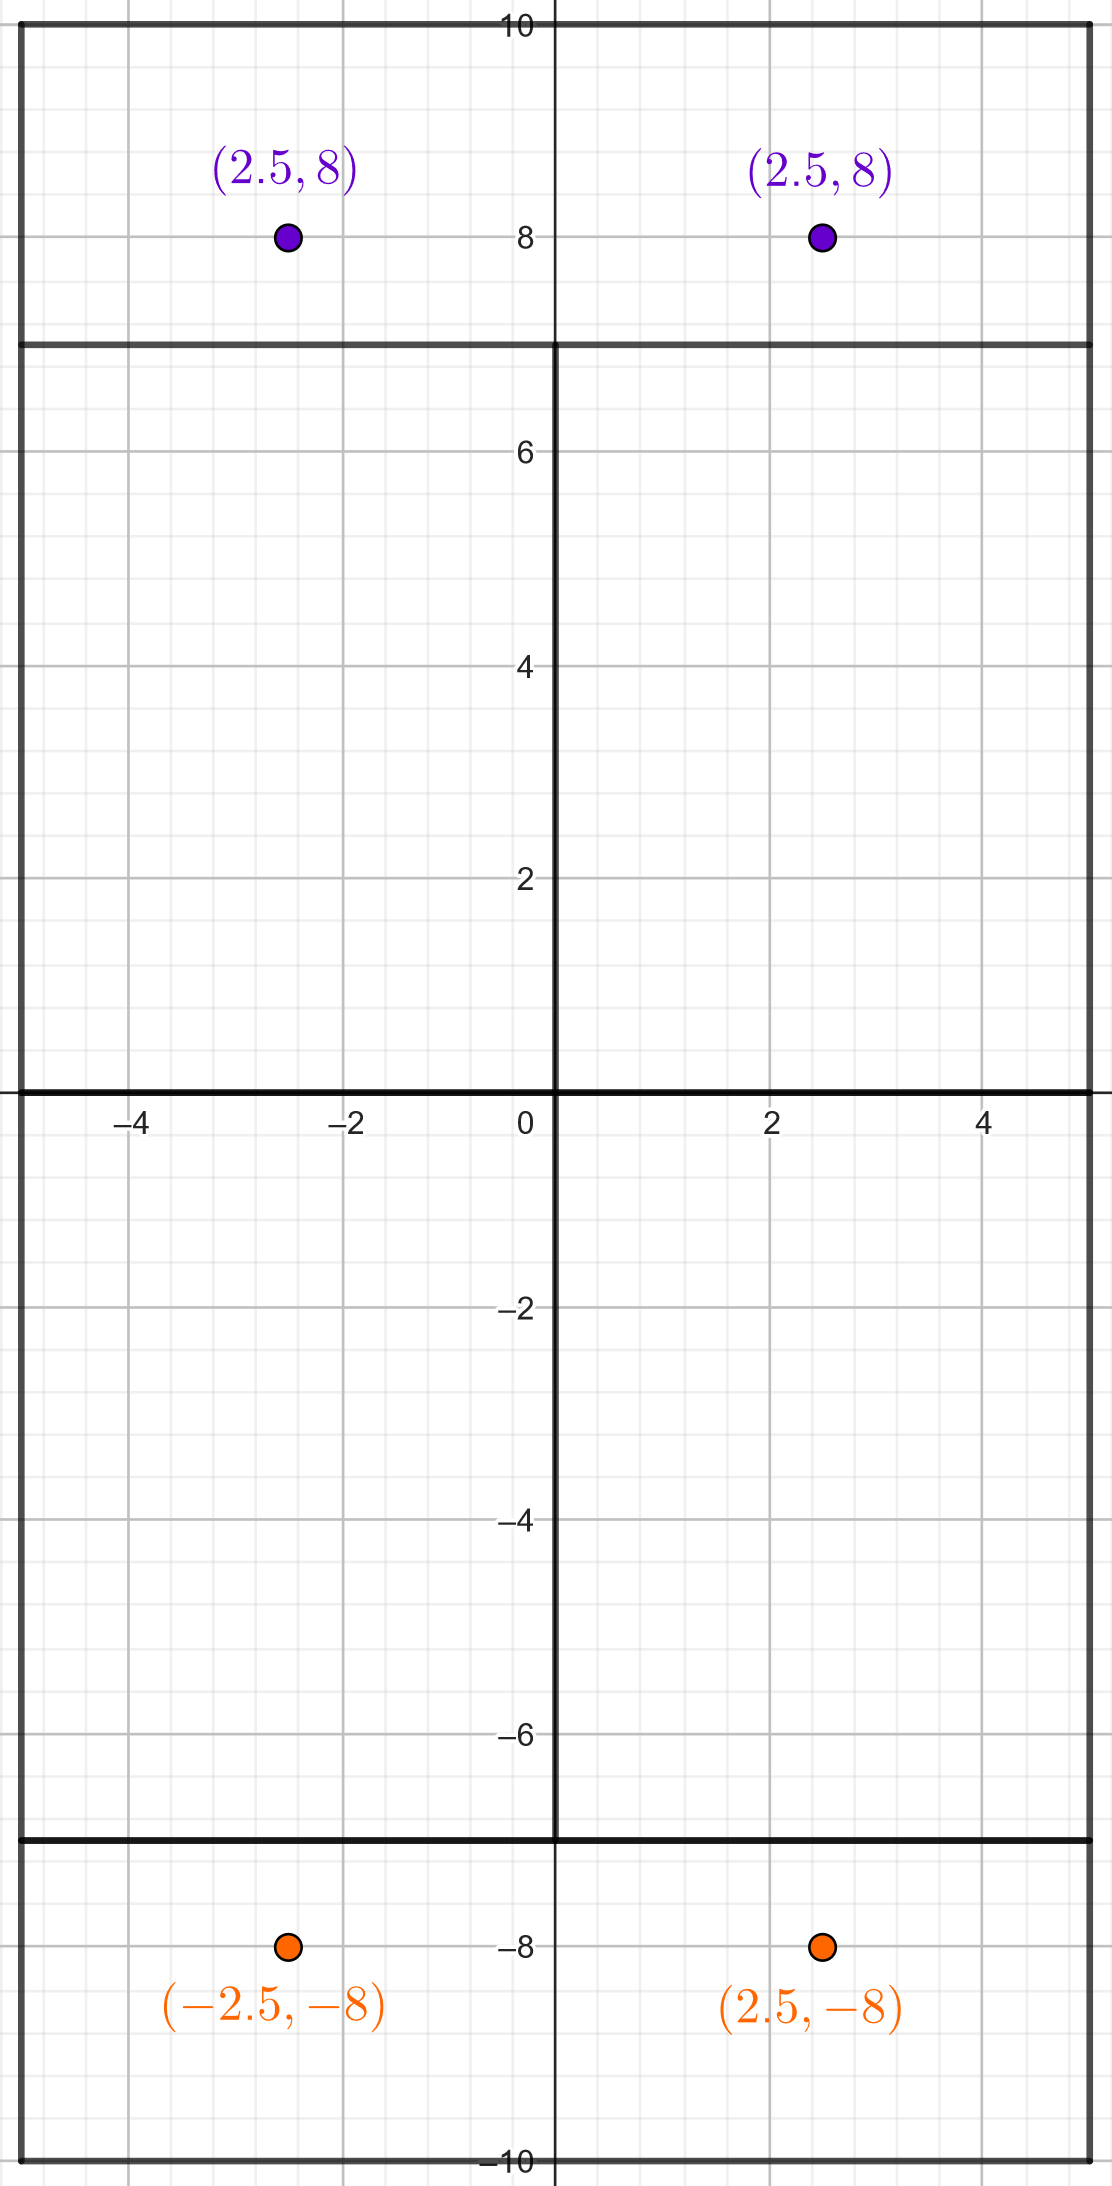
\includegraphics[width=7.5cm]{figures/serve-positions.png}
    \caption[Posiciones de servicio del entorno virtual de pádel]{Posiciones de servicio del entorno virtual de pádel. (Elaboración propia)}
    \label{fig:serve-positions}
\end{figure}

\subsubsection{Controlador de la pelota}

En el controlador de la pelota se han implementado todas aquellas funcionalidades relacionadas con la pelota, como el golpeo de la pelota, ya sea para saques o devoluciones, o el control sobre impactos y rebotes, tanto en el suelo como en la pared, entre otros.

Para golpear la pelota se calcula el cambio de velocidad necesario para que impacte en una determinada posición, dada una posición inicial, una altura máxima y el equipo del jugador que pretende golpearla. La posición de impacto es una selección de una de las posiciones de la cuadrícula de posiciones la pista. Esta cuadrícula tiene una resolución de $5\times5$, dejando una separación equidistante de $\frac{10}{6}$ metros entre cada posición, tal y como se muestra en la Figura \ref{fig:grid-padel}. 

\begin{figure}[H]
    \centering
    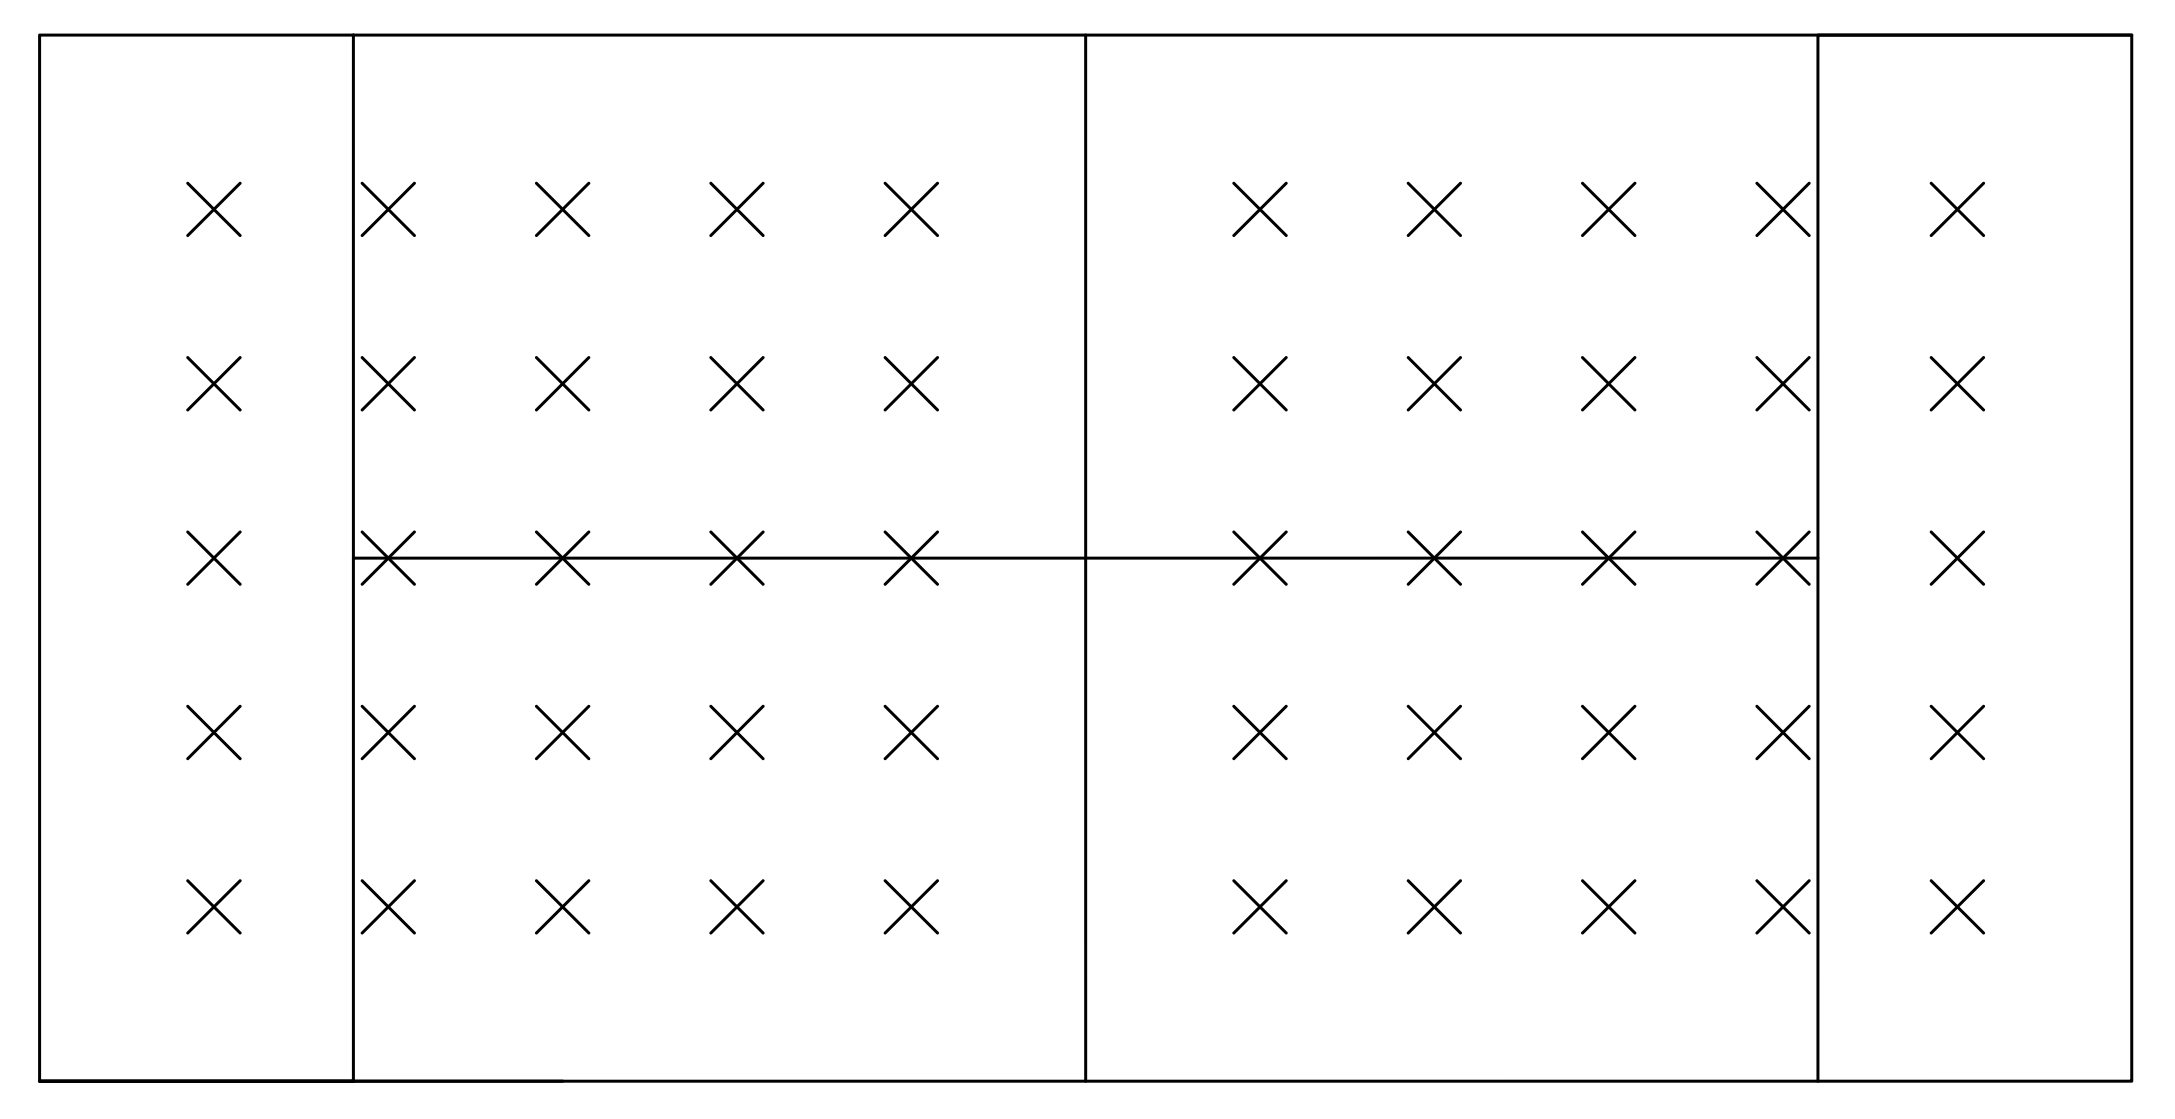
\includegraphics[width= 15cm]{figures/grid-padel.jpg}
    \caption[Cuadrícula de la pista de padel]{Cuadrícula de la pista de padel. Cada cruz representa una posición de impacto, equidistantes entre sí a una distancia de $\frac{10}{6}$ metros. (Elaboración propia)}
    \label{fig:grid-padel}
\end{figure}

Desde el punto de vista de cada equipo, la posición $(0, 0)$ de la cuadrícula corresponde a la esquina superior izquierda del campo contrario, la posición $(4, 0)$ a la esquina superior derecha, la posición $(0,4)$ a la esquina inferior izquierda, cerca de la red, y la posición $(4,4)$ a la esquina inferior derecha, también cerca de la red. Esto permite reducir la complejidad del aprendizaje, aprovechando una vez más la simetría del pádel. Por ejemplo, para la misma colocación de los oponentes desde el punto de vista de un jugador, la posición óptima de impacto debería ser la misma independientemente de si es de un equipo u otro. Por supuesto, esto es válido siempre y cuando las observaciones de los agentes también estén invertidas.

Para el cálculo de la fuerza se utilizan las ecuaciones de movimiento parabólico:
\begin{equation}
    x = x_0 + v_x + t
\end{equation}
\begin{equation}
    y = y_0 + v_{y_0} t + \frac{1}{2} a t^2
    \label{eq:mrua-y}
\end{equation}
\begin{equation}
    v_x = v_{x_0}
\end{equation}
\begin{equation}
    v_y = v_{y_0} + a t
\end{equation}
donde $x$ y $v_x$ son las ecuaciones de movimiento rectilíneo uniforme (MRU) en el eje $X$, e $y$ y $v_y$ las ecuaciones de movimiento rectilíneo uniformemente acelerado en el eje $Y$. Nótese que para el eje $Z$ también se utilizan las ecuaciones de MRU, pero se omite por simplificación al ser equivalentes a las del eje $X$.

El uso de las ecuaciones de movimiento parabólico se trata de una simplificación respecto al comportamiento real, ya que se ignora la fricción de la pelota con el aire, así como los diferentes efectos que pueden acompañar al golpeo (cortado, liftado, spin lateral).

Los datos disponibles son la posición inicial $(x_0, y_0, z_0)$, la posición final $(x_f, 0, z_f)$ (es decir, el objetivo para la pelota que ha elegido el agente), la aceleración $a = -9.8 \, \text{m/s}^2$ y la altura máxima $y_{max}$. Bajo estas condiciones, es posible calcular las velocidades iniciales $(v_{x_0}, v_{y_0}, v_{z_0})$ desarrollando las ecuaciones de movimiento parabólico. 

Dado que cuando la altura es máxima, la velocidad $v_y = 0$, y por lo tanto $t = -\frac{v_{y_0}}{a}$:
\begin{equation}
\begin{split}
    y_{max} &= y_0 + v_{y_0} t + \frac{1}{2} a t^2  \\
     &= y_0 + v_{y_0} \left(-\frac{v_{y_0}}{a}\right) + \frac{1}{2} a \left(-\frac{v_{y_0}}{a}\right)^2 \\
     &= y_0 - \frac{v_{y_0}^2}{2a} \\
    v_{y_0} &= \sqrt{(y_0 - y_{max}) 2 a}
\end{split}
\label{eq:y-max-calc}
\end{equation}
Para calcular las velocidades iniciales en los ejes $X$ y $Z$, es necesario calcular el tiempo total desde el instante en el que se golpea la pelota hasta que cae al suelo. Este tiempo se puede calcular sustituyendo $v_{v_0}$, obtenido a partir de la Ecuación \ref{eq:y-max-calc}, en la Ecuación \ref{eq:mrua-y}. Resolviendo la ecuación de segundo grado para $t > 0$, se obtiene el tiempo necesario para calcular $v_{x_0}$ y $v_{z_0}$:
\begin{equation}
    v_{x_0} = \frac{x_f - x_0}{t}
\end{equation}
\begin{equation}
    v_{z_0} = \frac{z_f - z_0}{t}
\end{equation}

En cuanto a las colisiones de la pelota, las cuales engloban el rebote y el impacto en otros objetos del entorno, se gestionan de la siguiente manera:
\begin{enumerate}
    \item[-] Cuando la pelota impacta en la red, si ha sido un impacto directo, el equipo que haya golpeado la pelota pierde el punto. Si ha sido un impacto después de que la pelota haya botado en el suelo del campo contrario, entonces este equipo gana el punto.
    \item[-] Cuando la pelota colisiona con otros jugadores tras la devolución de un cierto jugador, si la pelota impacta en un jugador del mismo equipo (ya sea a sí mismo o a su compañero), su equipo pierde el punto. Si impacta en un jugador del equipo contrario, se considera que los oponentes no han sido capaces de devolverla, por lo que su equipo gana el punto.
    \item[-] Para los rebotes en la pared tras la devolución de un cierto jugador, si ha sido un impacto directo en la pared del campo contrario, su equipo pierde el punto. Si durante el servicio toca la malla tras el primer rebote en el suelo, también pierde el punto.
    \item[-] Para los rebotes en el suelo, si la pelota ha rebotado por segunda vez sin haberse cometido ninguna falta, gana el punto el equipo que la haya golpeado. Si se trata del primer rebote, si es durante el servicio y la pelota bota fuera del área correspondiente, el equipo que haya realizado el servicio pierde el punto. Si no es durante el servicio, un equipo pierde el punto cuando golpea la pelota pero esta rebota en el campo propio.
\end{enumerate}
Cada vez que se gana un punto, el controlador de la pelota reinicia el estado de la pelota y solicita al controlador del entorno que sume un punto al equipo correspondiente. Es entonces cuando el controlador del entorno hace las llamadas pertinentes para reiniciar todo el entorno.

Otro aspecto a tener en cuenta es la sincronización de la pelota con el entorno, ya que muchas de las funciones se ejecutan de forma concurrente, en respuesta a eventos. En ocasiones, tras la devolución de la pelota, mientras se calcula predicción de la trayectoria de la pelota para el modo depuración, es posible que un jugador del equipo contrario devuelva la pelota antes de que haya finalizado el cálculo, creando incoherencias en las fuerzas aplicadas. Para evitar esto, cuando empieza el cálculo de la predicción se bloquea la pelota durante un margen de 0.1 segundos.

Otra situación problemática se da cuando, durante el reinicio del entorno, un jugador se encuentra justamente en la posición donde se debe colocar la pelota, haciendo que se juegue un punto indeseado. Para impedir que pase esto, tras finalizar un punto, la pelota se coloca en una posición fuera de la pista y se mantiene ahí durante un margen de 0.1 segundos, para que todos los jugadores puedan recolocarse correctamente, y entonces colocar la pelota en la posición correspondiente.

El resto de funcionalidades sirven para gestionar el estado de la pelota, por ejemplo para reiniciar el estado de la pelota, cambiar el color del \texttt{Trail Renderer} tras cada golpeo, colocar la pelota delante del servidor, etc.

\subsubsection{Controlador de la trayectoria}

El controlador de la trayectoria se utiliza para simular la trayectoria de la pelota tras cada golpeo. Este controlador crea una escena de físicas de Unity (esto es, una escena de Unity que utiliza únicamente el motor físico de Unity y permite hacer simulaciones de interacciones físicas entre objetos) para cada entorno, replicando los \texttt{Colliders} de la pista del entorno correspondiente, y utiliza una réplica de la pelota para simular su trayectoria con un número determinado de frames de antelación.

En cada simulación, se instancia una réplica de la pelota, denominada \texttt{GhostBall}, en una determinada posición inicial, y se le aplica un determinado cambio de velocidad. La escena de físicas simula un frame cada vez que se hace una llamada al método \texttt{PhysicsScene.Simulate(float step)}, dado un cierto intervalo de tiempo, normalmente definido por un intervalo de tiempo fijo \texttt{Time.fixedDeltaTime}. La idea es, por lo tanto, hacer llamadas reiterativamente hasta un número máximo de frames, o bien hasta cuando la pelota haya llegado a un estado terminal (es decir, que haya rebotado dos veces en el suelo). Esto permite simplificar la predicción de la trayectoria de la pelota, eliminando la necesidad de calcular los cambios de velocidad tras los rebotes.

Durante la simulación, las posiciones de la réplica de la pelota en cada frame de la escena de físicas se envía al controlador de posiciones clave, ya que algunas posiciones de interés que se han definido tienen relación con la trayectoria de la pelota. Concretamente para el modo de depuración, cuando está activado, estas mismas posiciones se utilizan también para determinar los puntos que conectan un \texttt{LineRenderer}, permitiendo de esta manera visualizar la trayectoria de la pelota. El \texttt{LineRenderer} se elimina cada vez que empieza una simulación nueva o bien cuando se desactiva el modo de depuración.

\subsubsection{Controlador de las posiciones clave}

El controlador de las posiciones clave define todas las posiciones de interés del entorno, las cuales pueden ser de devolución o de cobertura, como se verá más adelante. Estas posiciones permiten asignar recompensas a los agentes cuando se encuentran cerca o están acercándose a las posiciones en cuestión. Utilizando estas recompensas durante el entrenamiento, el objetivo es que los agentes puedan aprender a posicionarse correctamente durante un partido de pádel siguiendo un criterio definido manualmente.

\newpage

Las posiciones de interés de devolución son relevantes para el rol \texttt{Receiver}, y se definen como aquellas posiciones por las que pasará la pelota y son alcanzables por uno de los jugadores del equipo correspondiente, antes de que la pelota sobrepase esa posición. Al haber muchas posiciones que cumplen este criterio, se ha decidido limitar el número de posiciones a un máximo de cinco posiciones.

Utilizando la misma distancia equidistante de la cuadrícula de posiciones, de $\frac{10}{6}$ metros, se divide un campo en intervalos en los que puede haber como mucho una única posición de interés. Cuando se envía la pelota del campo de T1 hasta el de T2, por ejemplo, dado un índice $0 \leq i < 5$, los intervalos se calculan como $z \in [(i + 1) \frac{10}{6}, (i + 2)\frac{10}{6})]$, empezando el primer intervalo a $\frac{10}{6}$ metros después la red, y terminando el último intervalo justo en la pared de la pista, a 10 metros después de la red. Si es una pelota que se envía del campo de T2 hasta el de T1, se hace exactamente lo mismo pero invirtiendo el eje $Z$. La posición de interés que se asigna a un intervalo es la primera que cumpla el criterio establecido, siguiendo el orden de la trayectoria, de más próximo a más lejano.

\begin{figure}[H]
    \centering
    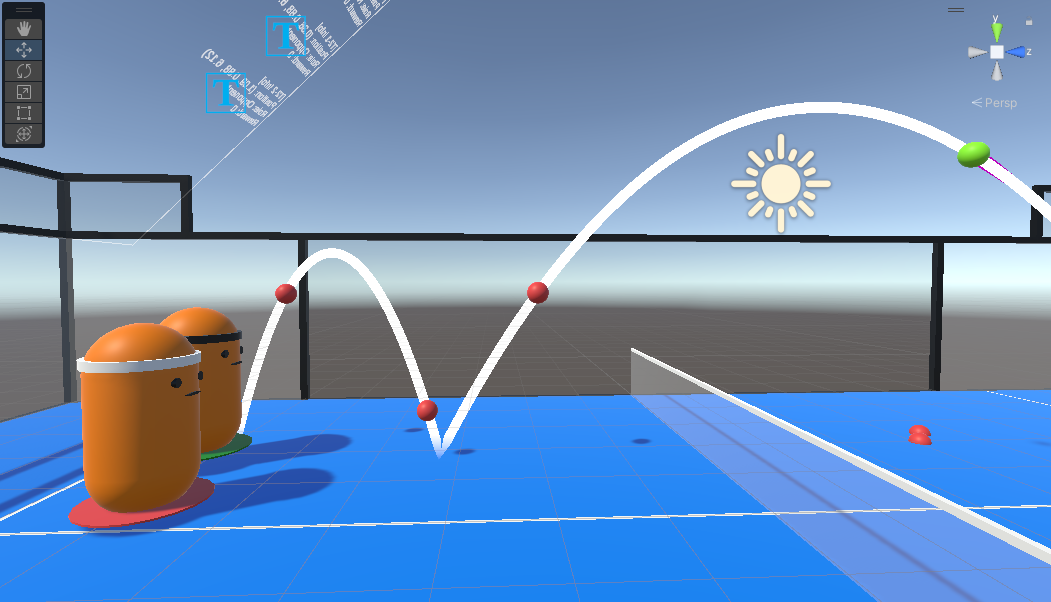
\includegraphics[width=13cm]{figures/receiver-keypoints.png}
    \caption[Posiciones de interés de devolución]{Posiciones de interés de devolución, representadas con un punto rojo en la línea de la trayectoria. En esta situación, el jugador 2 del equipo T1 (cinta negra) ha recibido el rol de \texttt{Receiver}, representado con la marca verde, ya que tiene más posiciones clave cerca. (Elaboración propia)}
    \label{fig:receiver-keypoints}
\end{figure}

Estas posiciones se calculan en el momento que se simula una trayectoria, ya que las posiciones futuras de la pelota provienen del controlador de la trayectoria. Una vez calculadas, se determina a quién se debería asignar el rol de \texttt{Receiver}, según qué jugador tiene más posiciones de interés de devolución más cercanas que el compañero. Las posiciones deben actualizarse constantemente, ya que a medida que pasa el tiempo pueden pasar a ser inalcanzables, ya sea porque la pelota haya sobrepasado la posición en cuestión, o bien porque ya no haya ningún jugador que pueda alcanzarla en el margen de tiempo restante. Como consecuencia, es posible que el rol de \texttt{Receiver} se vaya alternando dinámicamente.

Mediante las posiciones clave de devolución, es posible definir una función de recompensa que incentiva al agente con mayor probabilidad de poder realizar una devolución a posicionarse correctamente para la devolución, ayudándole de cierta manera a predecir dónde caerá la pelota.

Las posiciones de interés de cobertura son relevantes para los roles \texttt{Teammate} y \texttt{Opponent}. El rol \texttt{Teammate} se asigna al compañero del agente que tenga el rol \texttt{Receiver}, y el rol \texttt{Opponent} se asigna a los agentes del equipo que acaba de devolver la pelota.

Una posición de cobertura consiste en la posición que cubre la zona más descubierta de un jugador. Dada la situación ilustrada en la Figura \ref{fig:coverage-example}, donde se sitúa el jugador $Player$ en la posición $(x, z) = (2, 7)$, en un área equivalente al campo del equipo T2, la posición de cobertura óptima se calcula como el punto medio de las distancias más largas entre el jugador y los límites del área:
\begin{equation}
    (x, z)_{KP} = (x, z)_{Player} + {0\text{.}5} \arg\max(\|\overrightarrow{x_1}\|, \|\overrightarrow{x_2}\|) + {0\text{.}5} \arg\max(\|\overrightarrow{z_1}\|, \|\overrightarrow{z_2}\|)
\end{equation}

\begin{figure}[H]
    \centering
    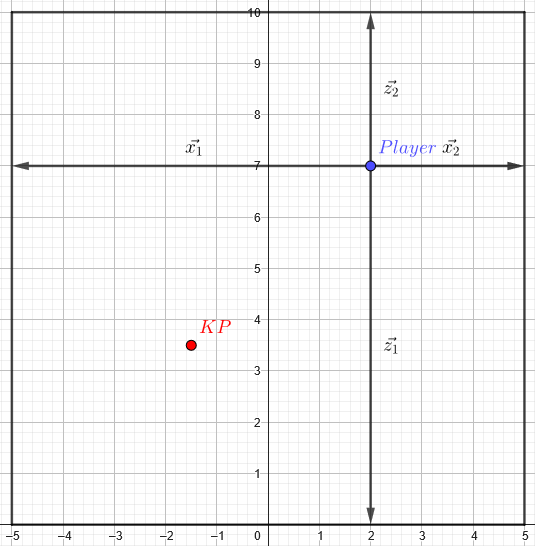
\includegraphics[width=10cm]{figures/coverage-example.png}
    \caption[Ejemplo de una posición óptima de cobertura]{Ejemplo de una posición óptima de cobertura $KP$, generada por el jugador $Player$. (Elaboración propia)}
    \label{fig:coverage-example}
\end{figure}

Estas posiciones de cobertura permiten incentivar a los agentes a distribuirse correctamente en la pista, evitando que los agentes de un mismo equipo se junten demasiado. En el caso del agente con el rol \texttt{Teammate} asignado, tendería a cubrir la zona que deja descubierta el agente \texttt{Receiver}. Para los agentes \texttt{Opponent} el comportamiento es distinto, ya que ambos  deberían cubrir el espacio descubierto que deja el otro agente. En este caso, los agentes tenderían a buscar un punto de equilibrio en el que ambos puedan cubrir su campo de manera óptima.

Por supuesto, en un partido real de pádel el punto óptimo para cubrir el espacio depende de diversos aspectos, no únicamente de las posiciones de los jugadores en el propio campo, pero se ha optado por utilizar una funcionalidad más simple para no aumentar demasiado la complejidad de la solución. El fin de utilizar estas posiciones de cobertura es, principalmente, para que los agentes aprendan que deben mantenerse alejados entre sí, pero sin que sea demasiado exagerado.

\begin{figure}[H]
    \centering
    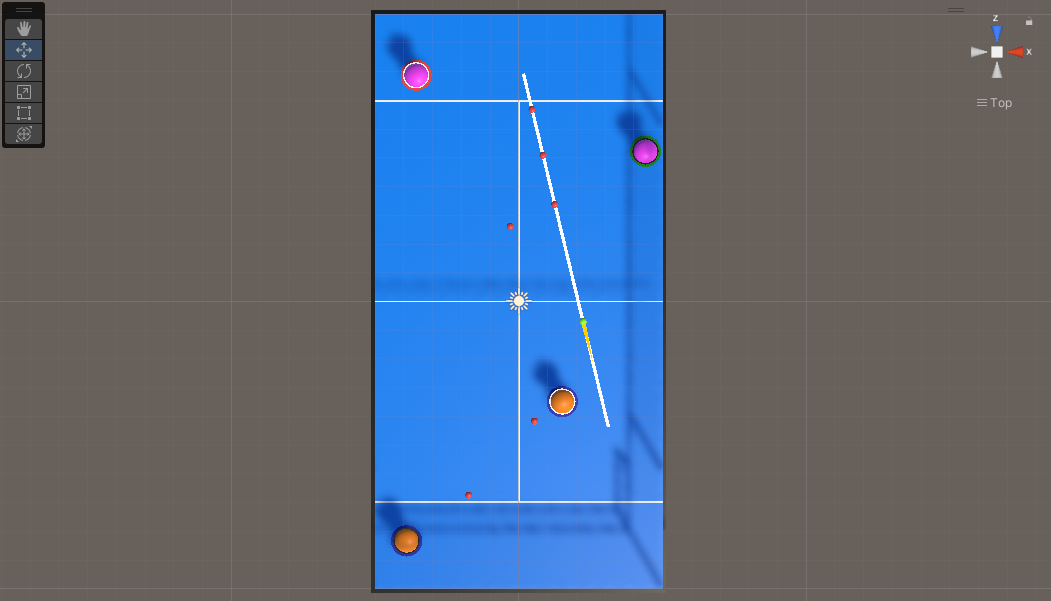
\includegraphics[width=13cm]{figures/coverage-key-positions.png}
    \caption[Posiciones de interés de cobertura]{Posiciones de interés de devolución, representadas con un punto rojo en el suelo de la pista. Ambos jugadores con el rol \texttt{Opponent} generan una posición de cobertura para el otro. El jugador con el rol \texttt{Receiver} genera una posición de cobertura para su compañero, con el rol \texttt{Teammate}. (Elaboración propia)}
    \label{fig:coverage-keypoints}
\end{figure}

En el controlador de las posiciones clave se implementan también los métodos utilizados para asignar roles y recompensas a los agentes. Para los roles, el rol de \texttt{Opponent} se asigna en el momento del golpeo, mientras que los roles \texttt{Receiver} y \texttt{Teammate} se asignan dependiendo de los puntos de devolución que se hayan calculado, y pueden ir alternándose dinámicamente.

Como ya se ha mencionado previamente, las recompensas se asignan a un agente cuando se está acercando o está cerca de un punto clave. Para comprobar si se está acercando, guarda internamente las posiciones del paso anterior y compara con el paso actual las distancias que hay entre ambas posiciones y la posición clave. Las posiciones de cobertura son únicas para los agentes correspondientes, y en el caso de las posiciones de devolución, se elige la posición más cercana al agente \texttt{Receiver}. Se considera que un agente está cerca de una posición clave cuando está a una distancia inferior a 1.5 metros.

\subsubsection{Agente de pádel}

El nuevo espacio de observaciones del agente de pádel consiste ahora en:
\begin{enumerate}
    \item[-] Las posiciones 2D de los cuatro agentes del entorno.
    \item[-] La posición y la velocidad 3D de la pelota.
    \item[-] Su propio rol, el cual puede ser \texttt{Opponent}, \texttt{Receiver} o \texttt{Teammate}.
    \item[-] Un valor booleano que indica si puede golpear la pelota.
\end{enumerate}
Sumando un total de 16 observaciones. En el caso de los agentes del equipo T2, se invierten las coordenadas del eje $X$ e $Z$, como ya se había mencionado en los cambios realizados.

\newpage

Un agente puede golpear la pelota cuando:
\begin{enumerate}
    \item[-] La pelota esta está a su alcance, dentro de un radio de 2 metros.
    \item[-] La pelota tiene una altura superior a 0.25 metros.
    \item[-] El último equipo en golpear la pelota ha sido el equipo contrario al del agente.
    \item[-] La pelota no está bloqueada debido al cálculo de simulaciones.
\end{enumerate}

El nuevo espacio de acciones está formado únicamente por acciones discretas, con un total de 5 ramas, donde cada rama consiste en un conjunto de subacciones de tamaño variable:
\begin{enumerate}
    \item[-] La rama 0, de tamaño 3, utilizada para definir el movimiento vertical: 0 para quedarse quieto, 1 para moverse hacia adelante, y 2 para moverse hacia atrás, dependiendo siempre de la orientación del agente (en esta versión, el agente solo puede tener dos orientaciones: 0º y 180º, que no cambian durante un juego).
    \item[-] La rama 1, de tamaño 3, utilizada para definir el movimiento horizontal: 0 para quedarse quieto, 1 para moverse hacia la derecha, y 2 para moverse hacia la izquierda, dependiendo también de la orientación del agente.
    \item[-] La rama 2, de tamaño 5, utilizada para especificar hacia qué columna de la cuadrícula enviar la pelota (representan cambios el eje X).
    \item[-] La rama 3, de tamaño 5, utilizada para especificar hacia qué fila de la cuadrícula enviar la pelota (representan cambios en el eje Z).
    \item[-] La rama 4, de tamaño 4, utilizada para especificar qué tipo de golpeo realizar: 0 para no golpear, 1 para ejecutar una derecha, 2 para un globo y 3 para un remate. Para una derecha se define una altura máxima $y_{max} = 2~\text{metros}$, para el globo $y_{max} = 4~ \text{metros}$ y para el remate $y_{max} = -1~\text{metros}$ (ya que en el cálculo de la velocidad inicial necesaria, cuando $y_{max} < y_0$, se asigna $y_{max} = y_0$ de manera que se aplica una velocidad paralela al plano $XZ$).
\end{enumerate}

El movimiento tanto vertical como horizontal se realiza con una velocidad de $5~\text{m/s}$ y depende del tiempo entre frames \texttt{Time.deltaTime}. Para el golpeo de la pelota se comprubea que el agente pueda golpearla dadas las condiciones descritas previamente. Tras el golpeo de la pelota, se añade una recompensa a nivel de equipo.

Este espacio de acciones no tiene por qué ser necesariamente este, pero debido a la limitación de tiempo del TFG, se ha dado por bueno y no se ha explorado más alla de este espacio. Sería posible aumentar la resolución de la cuadrícula y añadir más tipos de golpeos, aunque esto aumentaría la complejidad del entrenamiento y requeriría más pasos de entrenamiento.

El inicio de un episodio comienza con el servicio y termina con la obtención de un punto. Al principio de cada episodio, los agentes no pueden moverse hasta que se haya realizado el servicio.

Las funciones de recompensa se han mencionado a lo largo de esta sección pero, resumidamente, un agente puede recibir una recompensa (o penalización, si es negativa) tras ganar un punto, perder un punto, acercarse a una posición clave, quedarse cerca de una posición clave o golpear a la pelota.

En el agente de pádel también se han implementado funcionalidades para modificar el estado del agente, por ejemplo para asignar los roles, cambiar el color de la marca según el rol, etc.

\subsection{Implementación específica para la grabación de demostraciones}

Además del entorno en todo su conjunto, también se han implementado las funcionalidades necesarias para la grabación de demostraciones, las cuales son necesarias para entrenar agentes mediante GAIL.

Con ML-Agents, las demostraciones normalmente son sencillas de obtener cuando se trata de entornos en los que hay un único agente. Durante la grabación, suele ser el propio usuario quien proporciona las demostraciones expertas mediante una heurística definida manualmente (por ejemplo, mover el agente mediante controles de teclado). En este entorno, sin embargo, al haber cuatro agentes que deben actuar como expertos, es díficil controlarlos a la vez a través de un teclado, y más aún si deben moverse de manera distinta, cuando todos comparten la misma heurística.

La solución que se ha propuesto para grabar las demostraciones es utilizar un conjunto de datos de partidos profesionales de pádel, obtenidos mediante la aplicación de técnicas de visión por computador para el seguimiento de los jugadores en vídeos de partidos \cite{s21103368}.

En esta solución, un \emph{entrenador} se encarga de procesar los datos relevantes del conjunto de datos, formando, en particular, muestras con información sobre una situación posicional y las acciones que hayan realizado los jugadores profesionales en cada respectiva situación. La idea es que un agente pueda solicitar al entrenador las acciones que debería realizar enviándole la información relevante del estado del entorno virtual. El entrenador, a partir de esta información, busca la muestra con la situación posicional más parecida posible dentro del conjunto de datos. La acción obtenida a partir de esta muestra se envía finalmente al agente para que la ejecute. Repitiendo esto sucesivamente, en cada paso, el objetivo es poder reproducir, en los agentes, un comportamiento similar a los jugadores profesionales en un partido de pádel.

Al igual que en el resto del entorno, la comunicación entre el agente y el entrenador se hace a través de un controlador del entrenador, con tal de evitar introducir dependencias entre estas clases.

\subsubsection{Entrenador}

El entrenador es un script de Python que funciona como un servidor, en el que se define un socket para establecer una comunicación con la aplicación de Unity. Este script carga el conjunto de datos especificado, lo procesa eliminando aquella información innecesaria y se queda en espera para recibir solicitudes. Estas solicitudes pueden ser de dos tipos, según si es para solicitar un movimiento, o bien para solicitar un golpeo. Cada solicitud llega acompañada de información sobre el estado del entorno virtual de pádel, y se utiliza para obtener la muestra más parecida del conjunto de datos según cómo de parecida sea la situación posicional con el estado del entorno virtual. A partir de esta muestra, se extrae la acción asociada y se devuelve finalmente al cliente.

El conjunto de datos que procesa el entrenador es, en particular, un fichero Excel (\texttt{.xslx}) que contiene 22,615 filas, donde cada fila consiste en la información posicional de los jugadores y de la pelota en una pista de pádel, además de otros valores calculados durante el posprocesamiento.

\newpage

En el dominio de estos datos, el origen de coordenadas $(0, 0)$ se sitúa en la esquina inferior izquierda de la pista, el ancho de la pista está definido por $x \in [0, 10]$, y el largo por $y \in [0, 20]$. Los jugadores situados en la mitad superior de la pista ($y > 10$) forman el equipo \texttt{T}, mientras que aquellos situados en la mitad inferior ($y < 10$) forman el equipo \texttt{B}. Dentro de un mismo equipo también se hace una distinción entre los propios jugadores, según en qué lado han empezado un punto. El jugador que está más a la izquierda se denomina \texttt{TL}, mientras que el jugador situado más a la derecha se denomina \texttt{TR}. Los jugadores del equipo B también se distinguen de esta manera, denominados \texttt{BL} y \texttt{BR}. En la Figura \ref{fig:dataset-plot} se representa una muestra individual en una gráfica, limitada por las medidas de una pista de padel.

\begin{figure}[H]
    \centering
    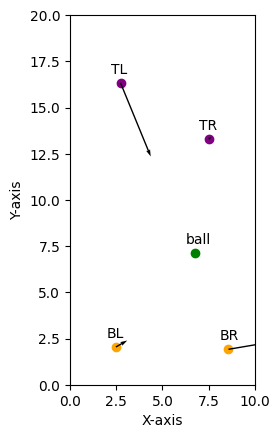
\includegraphics[width=5cm]{figures/dataset-plot.png}
    \caption[Ejemplo gráfico de una única muestra del conjunto de datos utilizado para grabar demostraciones]{Ejemplo gráfico de una única muestra del conjunto de datos utilizado para grabar demostraciones. (Elaboración propia)}
    \label{fig:dataset-plot}
\end{figure}

Los valores relevantes de este conjunto de datos, además de algunos ejemplos de muestras, se presentan en la Figura~\ref{fig:dataset-raw}. De izquierda a derecha, cada par (\texttt{x}, \texttt{y}) consiste en la posición de un jugador \texttt{TL}, \texttt{TR}, \texttt{BL}, \texttt{BR}, respectivamente; \texttt{(ball x, ball y)} es la posición de la pelota; cada par (\texttt{speedx}, \texttt{speedy}) es la velocidad de cada respectivo jugador; \texttt{shot} es el tipo de golpeo que se ejecuta, según si es un golpeo normal, un globo o un remate, definido únicamente en aquellas muestras en los que un jugador golpea la pelota; y \texttt{last hit} es una variable que indica qué equipo ha sido el último en golpear la pelota.

\begin{figure}[H]
    \centering
    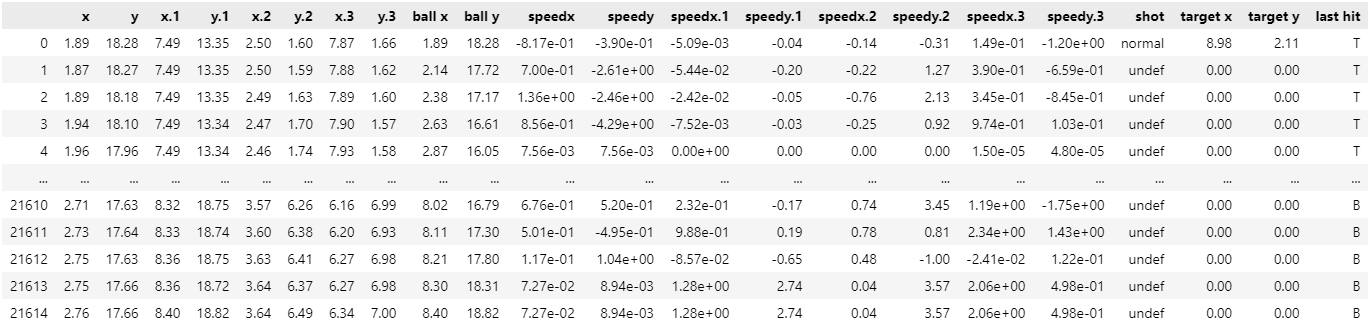
\includegraphics[width=\textwidth]{figures/data.png}
    \caption[Conjunto de datos utilizado para la grabación de demostraciones]{Conjunto de datos utilizado para la grabación de demostraciones. (Elaboración propia)}
    \label{fig:dataset-raw}
\end{figure}

A partir de estos valores, se define un subconjunto de valores que definen una situación posicional, formado por las posiciones de cada jugador y de la pelota:
\begin{center}
    [\texttt{x}, \texttt{y}, \texttt{x.1}, \texttt{y.1}, \texttt{x.2}, \texttt{y.2}, \texttt{x.3}, \texttt{y.3}, \texttt{ball x}, \texttt{ball y}]
\end{center}
De esta manera, es posible definir que la muestra del conjunto de datos más parecida a un estado del entorno virtual es aquella cuyas posiciones son lo más cercanas posibles a las posiciones del estado del entorno virtual, dentro de un dominio común para ambos conjuntos y utilizando la distancia Euclídea, dado que todos estos datos están en metros.

Debido a que el entrenador puede recibir solicitudes distintas según si es para solicitar un movimiento o un golpeo, también se hace una separación en los espacios de búsqueda. Esto se ha decidido así porque para extraer información sobre el golpeo de una muestra, una condición necesaria es que el golpeo esté definido, es decir, que el valor de \texttt{shot} sea distinto a \texttt{undef}. Además de la separación entre datos de movimiento y datos de golpeo, dentro de cada conjunto es necesario hacer otra divisón según el valor categórico \texttt{last hit}. Esta división es importante para mantener la coherencia de los datos, ya que el movimiento de los jugadores es distinto según si la pelota está yendo al propio campo o al campo rival. De la misma manera, el golpeo también es distinto según si lo realiza un jugador del equipo \texttt{T} o del equipo \texttt{B}:
\begin{enumerate}
    \item Datos de movimientos cuando la pelota ha sido golpeada por el equipo \texttt{T}.
    \item Datos de movimientos cuando la pelota ha sido golpeada por el equipo \texttt{B}.
    \item Datos de golpeos realizados por el equipo \texttt{T}.
    \item Datos de golpeos realizados por el equipo \texttt{B}.
\end{enumerate}

Un algoritmo adecuado para realizar búsquedas de muestras bajo estas condiciones es mediante árboles decisionales, concretamente árboles \emph{k}-dimensionales. El entrenador, después de haber creado los subconjuntos de datos correspondientes aplicando los filtros necesarios, crea cuatro árboles \emph{k}-dimensionales, uno para cada subconjunto. Estos árboles permiten realizar búsquedas eficientes de los vecinos más próximos a una muestra proporcionada (en este caso, un vector 10-dimensional con el formato del subconjunto de valores que definen una
situación posicional).

Tras completar la búsqueda, el entrenador envía al entorno virtual de Unity una respuesta en un formato determinado, según el tipo de acción que se haya buscado. En el caso de haber consistido en una búsqueda de un golpeo, la trama contiene el tipo de golpeo realizado, además de la posición de impacto:
\begin{center}
    [\texttt{shot}, \texttt{target x}, \texttt{target y}]
\end{center}
Para una búsqueda de un movimiento, la trama consiste en cuatro posiciones, una para cada jugador, y el vector de velocidad de cada posición:
\begin{center}
    [\texttt{x}, \texttt{y}, \texttt{x.1}, \texttt{y.1}, \texttt{x.2}, \texttt{y.2}, \texttt{x.3}, \texttt{y.3}, \texttt{speedx}, \texttt{speedy}, \texttt{speedx.1}, \texttt{speedy.1}, \texttt{speedx.2}, \texttt{speedy.2}, \texttt{speedx.3}, \texttt{speedy.3}]
\end{center}

Específicamente para la comunicación entre el cliente y el servidor, las tramas que se intercambian también contienen otros valores que indican el tipo de solicitud (\texttt{SHOT\_REQUEST}, \texttt{MOVEMENT\_REQUEST}), el tipo de respuesta (\texttt{SHOT\_RESPONSE}, \texttt{MOVEMENT\_RESPONSE}), y el identificador \texttt{PlayerId} del jugador que haya enviado la solicitud o al que se quiera enviar la respuesta. Esto permite tanto al cliente como al servidor poder mantener un control sobre la comunicación, pudiendo diferenciar qué tipo de información tiene cada trama y hacia quién va dirigida. 

En las solicitudes de movimiento enviadas desde el entorno virtual al entrenador, también se especifica el último equipo que haya golpeado la pelota, según si ha sido \texttt{T1} o \texttt{T2}. Esto permite al entrenador determinar qué árbol utilizar para la búsqueda, asociando los equipos \texttt{T1} y \texttt{T2} del entorno virtual a los equipos \texttt{B} y \texttt{T} de los datos, respectivamente.

Para las solicitudes de golpeo no es necesario especificar el último equipo que haya golpeado la pelota, ya que se asume que el jugador que haya enviado la solicitud será el jugador que golpeará la pelota. Por lo tanto, basta con asociar los jugadores \texttt{T1\_1} y \texttt{T1\_2} con los datos de golpeos realizados por el equipo \texttt{B}, y los jugadores \texttt{T2\_1} y \texttt{T2\_2} con los datos de golpeos realizados por el equipo \texttt{T}.

\subsubsection{Heurística del agente}

Las solicitudes de movimientos y golpeos las envía el agente a través de la implementación de la heurística. Para moverse, se envían solicitudes de movimientos contínuamente. Para el golpeo de la pelota, se envían solicitudes de golpeos siempre y cuando la pelota esté dentro de un rango de golpeo. El agente realiza las acciones proporcionadas por el entrenador en el mismo instante que las recibe.

Tanto en las solicitudes de movimientos como de golpeos se envían su identificador, las posiciones locales del propio agente, de su compañero, de sus dos oponentes y de la pelota. En las solicitudes de movimientos se envía también la información sobre qué equipo ha golpeado la pelota por última vez.

Para no colapsar el intercambio de mensajes entre el agente y el entrenador, el agente tiene implementado un sistema de control no bloqueante para el envío de solicitudes y la ejecución de acciones. Un agente puede enviar una solicitud siempre y cuando no esté esperando a que llegue la respuesta de una solicitud pasada. En cuanto un agente recibe la acción que debe realizar, se considera que la solicitud pasada, que estaba pendiente a ser resuelta, ya se ha resuelto, por lo que el agente puede proceder a enviar la siguiente solicitud.

\subsubsection{Controlador del entrenador}

El controlador del entrenador sirve como intermediario entre el agente y el entrenador. Dado que el dominio de las posiciones en el entorno virtual de pádel es distinto al dominio del conjunto de datos de partidos profesionales de pádel, es necesario preprocesar los datos enviados desde el agente al entrenador, y posprocesar la información recibida del entrenador para enviársela al agente.

En el preprocesamiento de datos, es necesario respetar el orden de los valores que utiliza el entrenador para la búsqueda de movimientos o golpeos. Por ello, las posiciones recibidas por el agente se ordenan siguiendo el orden \texttt{TL}, \texttt{TR}, \texttt{BL} y \texttt{BR}, identificando primero qué posiciones forman parte del equipo de la parte superior \texttt{T} ($z > 0$), y de la parte inferior \texttt{B} ($z < 0$), para luego determinar, dentro de cada equipo, qué posición está más a la izquierda del otro, sin tener en cuenta orientaciones, para ordenar según los lados \texttt{T} y \texttt{R}. Además, se elimina el eje $Y$ de las posiciones ya que no se dispone de información sobre la altura en los datos del entrenador. Por último, se aplica una traslación a cada posición con un vector $\vec{v} = (x, z) = (5, 10)$, para transformar el dominio de las posiciones del estado del entorno virtual al dominio de los datos del entrenador.

\newpage

Por otro lado, en el posprocesamiento, lo primero que se hace es la traslación inversa $-\vec{v} = -(x, z) = (-5, -10)$ para proceder a adaptar la acción recibida del entrenador a una acción del entorno virtual.

Para el posprocesamiento de golpeos, la información de la que se dispone es el tipo de golpeo y la posición de impacto. La traducción del tipo de golpeo \texttt{shot}, los cuales pueden ser \texttt{normal}, \texttt{lob} o \texttt{smash}, es directa: los valores de la rama 4 serían 1, 2 o 3, respectivamente. Para la selección de la posición dentro de la cuadrícula de posiciones, la idea es que se asocie la posición de impacto con el punto de la cuadrícula que minimiza la distancia entre la posición de impacto y la posición local real de la cuadrícula. Para ello, se inicializa una matriz tanto para \texttt{T1} como para \texttt{T2}, para asignar la posición local real correspondiente a cada posición de la cuadrícula. Haciendo un recorrido sobre la matriz correspondiente, se calculan los índices de la cuadrícula que minimicen la distancia entre la posición de impacto y la posición local real de la cuadrícula, y de esta manera se obtienen los valores necesarios para la rama 2 y 3 de las acciones discretas del agente.

Antes de definir el posprocesamiento de movimientos, cabe mencionar que el envío de solicitudes de movimientos tienen un comportamiento especial. En el entorno virtual, si los cuatro agentes enviaran constantemente solicitudes de movimientos, prácticamente de manera simultánea, el entrenador recibiría la misma información y devolvería la misma muestra para cada agente, solo que con un vector de velocidad distinto. Esto no es un funcionamiento deseado, ya que es bastante ineficiente. En su lugar, cuando el controlador del entrenador recibe una solicitud de movimiento por parte del agente, bloquea el envío del resto de solicitudes de movimientos hasta que se resuelva la primera solicitud recibida. La respuesta a esta solicitud no se trata únicamente del vector de velocidad del agente que envió la solicitud originalmente, sino que contiene información sobre cuatro posiciones y sus respectivas velocidades. Utilizando toda esta información, es posible calcular las acciones para todos los agentes con una única búsqueda.

Para el posprocesamiento de movimientos, por lo tanto, dadas las cuatro posiciones y sus respectivas velocidades, el primer paso es asociar cada posición al agente correspondiente. Esto se hace fácilmente calculando qué agente está más cerca de cada posición. Asociando a un agente una determinada posición, también se asocia indirectamente la velocidad que debería tener, y esta velocidad es justamente lo que define el movimiento del agente. Dependiendo de la orientación de cada agente, se asignan algunos valores u otros dependiendo del signo de la velocidad en los ejes correspondientes. Por ejemplo, dado un agente del equipo \texttt{T1}, el cual tiene vectores \texttt{Forward} y \texttt{Right} orientados hacia los ejes positivos $Z$ y $X$, respectivamente, según el signo de la primera componente de la velocidad (eje $X$), debería moverse hacia la izquierda si fuera negativo, quedarse quieto si fuera 0, o moverse hacia la derecha si fuera positivo. Similarmente para la segunda componente, hacia adelante si fuera positivo, quedarse quieto si fuera 0, o hacia detrás si fuera negativo.

En la Figura \ref{fig:diagrama_coach} se muestra un diagrama secuencial de una ciclo completo de la comunicación entre el agente, el controlador del entrenador y el entrenador.

\begin{figure}[H]
    \centering
    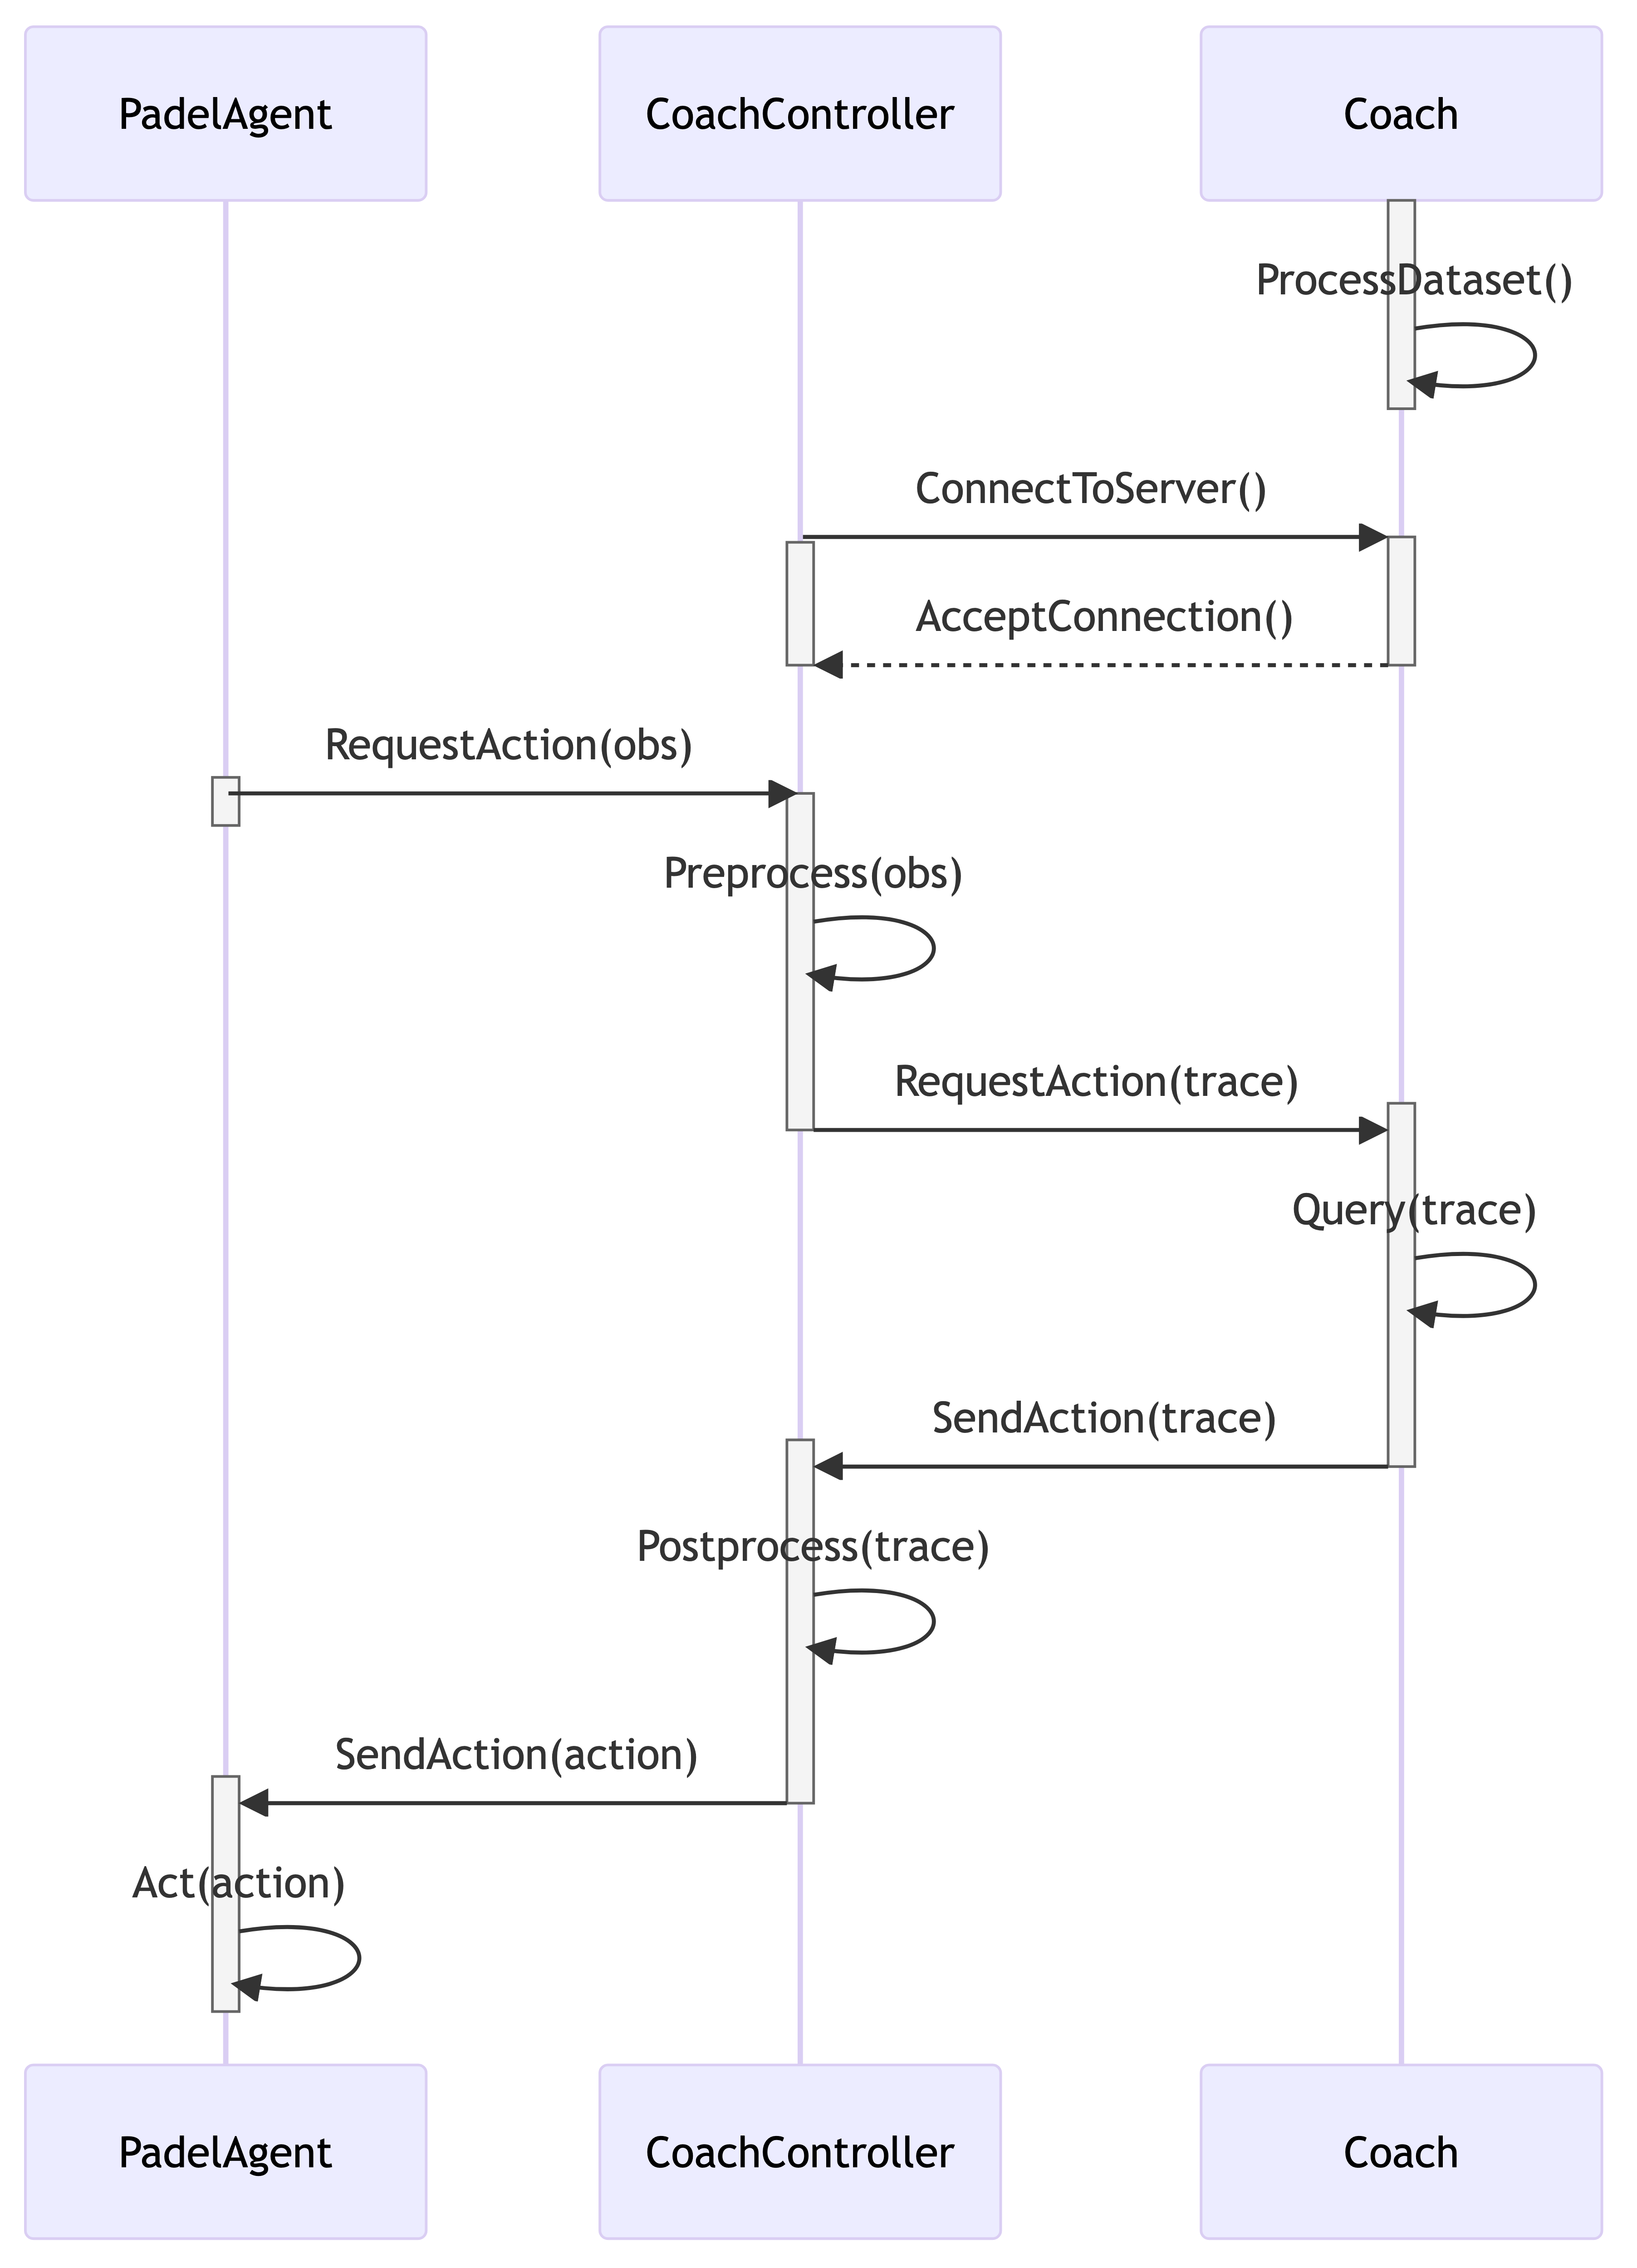
\includegraphics[width=12.5cm]{figures/diagrama_coach.png}
    \caption[Diagrama secuencial de la comunicación entre el agente, el controlador del entrenador y el entrenador]{Diagrama secuencial de la comunicación entre el agente, el controlador del entrenador y el entrenador. (Elaboración propia)}
    \label{fig:diagrama_coach}
\end{figure}